\documentclass[letterpaper]{article}
\usepackage{calc,amsmath,amssymb,amsfonts}
\usepackage[T1]{fontenc}
\usepackage[spanish,english]{babel}
\usepackage{xcolor,longfbox,fancyhdr}
\usepackage[top=0.9307in,bottom=0.1945in,left=0.9028in,right=0.9165in,nohead,includefoot,foot=12pt,footskip=18.6024pt]{geometry}
\usepackage{enumitem,hyperref}
\hypersetup{colorlinks=true,allcolors=blue,pdfauthor=Luis Angel Cruz Quispe}
\usepackage[pdftex]{graphicx}
\usepackage{tikz}
\makeatletter\newdimen\@tempdimd\makeatother
% Outline numbering
\setcounter{secnumdepth}{0}
% Text styles
\newcommand\textstyleListLabelxix[1]{\textrm{\textbf{#1}}}
\newcommand\textstyleStrong[1]{\textbf{#1}}
% Pages
\fancypagestyle{Convertedi}{\fancyhf{}
  \fancyhead[L]{}
  \fancyfoot[L]{\begin{tikzpicture}
\begin{scope}[xshift=10.672cm,yshift=-26.155cm]
\path  (NaN,NaN) --  (Infinity,NaN) --  (Infinity,-Infinity) --  (NaN,-Infinity) -- cycle;
\node[below,align=left,text width=NaNcm,transform shape] at (NaN,NaN) {1};
\end{scope}
\end{tikzpicture}
}
  \renewcommand\headrulewidth{0pt}
  \renewcommand\footrulewidth{0pt}
  \renewcommand\thepage{\arabic{page}}
}
\fancypagestyle{Standard}{\fancyhf{}
  \fancyhead[L]{}
  \fancyfoot[L]{}
  \renewcommand\headrulewidth{0pt}
  \renewcommand\footrulewidth{0pt}
  \renewcommand\thepage{\arabic{page}}
}
\fancypagestyle{Convertediv}{\fancyhf{}
  \fancyhead[L]{}
  \fancyfoot[L]{}
  \renewcommand\headrulewidth{0pt}
  \renewcommand\footrulewidth{0pt}
  \renewcommand\thepage{\arabic{page}}
}
\fancypagestyle{Convertediii}{\fancyhf{}
  \fancyhead[L]{}
  \fancyfoot[L]{\begin{tikzpicture}
\begin{scope}[xshift=10.513cm,yshift=-26.155cm]
\path  (NaN,NaN) --  (Infinity,NaN) --  (Infinity,-Infinity) --  (NaN,-Infinity) -- cycle;
\node[below,align=left,text width=NaNcm,transform shape] at (NaN,NaN) {\thepage{}};
\end{scope}
\end{tikzpicture}
}
  \renewcommand\headrulewidth{0pt}
  \renewcommand\footrulewidth{0pt}
  \renewcommand\thepage{\arabic{page}}
}
\fancypagestyle{Convertedii}{\fancyhf{}
  \fancyhead[L]{}
  \fancyfoot[L]{\begin{tikzpicture}
\begin{scope}[xshift=10.672cm,yshift=-26.155cm]
\path  (NaN,NaN) --  (Infinity,NaN) --  (Infinity,-Infinity) --  (NaN,-Infinity) -- cycle;
\node[below,align=left,text width=NaNcm,transform shape] at (NaN,NaN) {2};
\end{scope}
\end{tikzpicture}
}
  \renewcommand\headrulewidth{0pt}
  \renewcommand\footrulewidth{0pt}
  \renewcommand\thepage{\arabic{page}}
}
\pagestyle{Standard}
\author{Luis Angel Cruz Quispe}
\date{2024-06-25}
\begin{document}
\clearpage
\pagestyle{Standard}
{\centering\selectlanguage{spanish}\bfseries
Universidad \ Nacional \ de \ Ingenier$\acute{}$ıa
\par}

{\centering\selectlanguage{spanish}
\textbf{FACULTAD DE CIENCIAS}
\par}


\bigskip



\begin{center}
\lfbox[margin-bottom=0.0102in,margin-top=0mm,margin-right=0mm,margin-left=0mm,border-style=none,padding=0mm,vertical-align=top,raise=-0.4346in]{
\includegraphics[width=2.65in,height=3.3854in]{a0000-img001.png}}
\end{center}

\bigskip


\bigskip

{\centering\selectlanguage{spanish}\bfseries
Proyecto de Fundamentos De Programación
\par}

{\centering\selectlanguage{spanish}\bfseries
2024-I
\par}


\bigskip

{\selectlanguage{spanish}
\textbf{Integrantes:}}


\bigskip

{\selectlanguage{spanish}
Facultad de Ciencias {}- Escuela de Ingeniería Física - Mamani Benites Jimmy - 20211489D\textbf{ }}

{\selectlanguage{spanish}
Facultad de Ciencias - Escuela de Ingeniería Física - Rios Cusi David - 20230216J}

{\selectlanguage{spanish}
Facultad de Ciencias - Escuela de Ingeniería Física - Cruz Quispe Luis - 20221664C}
\clearpage
\pagestyle{Convertedi}

\bigskip


\bigskip


\bigskip


\bigskip


\bigskip


\bigskip


\bigskip


\bigskip

{\selectlanguage{spanish}
\textbf{Índice:}}


\bigskip

{\selectlanguage{spanish}
\textbf{1.\ \ Fundamento \ teórico}}


\bigskip

\begin{enumerate}[series=listWWNumxiii,label=\arabic*.,ref=\arabic*]
\item \begin{enumerate}[series=listWWNumxiii,label=\arabic{enumi}.\arabic*.,ref=\arabic{enumi}.\arabic*]
\item {\selectlanguage{spanish}
\foreignlanguage{english}{Librerias:}}
\end{enumerate}
\end{enumerate}

\bigskip

{\selectlanguage{spanish}
\foreignlanguage{english}{1.1.1.\ \ Pandas}}

{\selectlanguage{spanish}
\foreignlanguage{english}{1.1.2.\ \ Marplotlib}}

{\selectlanguage{spanish}
\foreignlanguage{english}{1.1.3.\ \ NumPy}}


\bigskip

{\selectlanguage{spanish}
\foreignlanguage{english}{1.2.\ \ Machine Learning}}

\foreignlanguage{english}{1.2.1.\ \ Scikit Learn}}

{\selectlanguage{spanish}
\foreignlanguage{english}{1.2.2.\ \ Por clasificación}}

{\selectlanguage{spanish}
1.3.\ \ Generación de textos}

{\selectlanguage{spanish}
1.4.\ \ Flask}

{\selectlanguage{spanish}
1.5.\ \ Selenium}


\bigskip


\bigskip

{\selectlanguage{spanish}
\textbf{2.\ \ Documentación clara y completa del código}}


\bigskip

{\selectlanguage{spanish}
2.1.\ \ Parte 1}

{\selectlanguage{spanish}
2.2.\ \ Parte 2}

{\selectlanguage{spanish}
2.3.\ \ Parte 3\ \ }

\clearpage
\pagestyle{Convertedii}

\bigskip


\bigskip


\bigskip


\bigskip


\bigskip


\bigskip


\bigskip


\bigskip


\bigskip


\bigskip


\bigskip


\bigskip


\bigskip


\bigskip


\bigskip


\bigskip


\bigskip

{\selectlanguage{spanish}
\textbf{Introduccio$\acute{}$n}}

{\selectlanguage{spanish}
Este proyecto \ explora \ herramientas \ y \ te$\acute{}$cnicas \ clave de \ ana$\acute{}$lisis \ de \ datos, \ machine
\ learning, \ procesamiento de \ lenguaje \ natural, \ desarrollo \ web \ y \ automatizacio$\acute{}$n. Utilizamos las
librer$\acute{}$ıas de Python Pandas, Matplotlib y \ NumPy \ para \ la \ manipulacio$\acute{}$n \ y
\ visualizacio$\acute{}$n \ de \ da- tos. Scikit-learn se emplea para implementar \ y \ eva- luar modelos de machine
learning. En procesamiento de \ lenguaje \ natural \ (NLP), \ aplicamos \ te$\acute{}$cnicas \ de \ cla-
sificacio$\acute{}$n \ \ de \ \ textos \ \ y \ \ generacio$\acute{}$n \ \ de \ \ contenido. \ \ Flask facilita \ \ el
\ \ desarrollo \ \ de \ \ aplicaciones \ \ web \ \ dina$\acute{}$micas, integrando modelos de machine learning.
Finalmente, Selenium automatiza pruebas y extraccio$\acute{}$n de datos web. Este enfoque integral combina diversas
tecnolog$\acute{}$ıas para resolver problemas complejos y desarrollar soluciones innovadoras.}

\clearpage
\pagestyle{Convertediii}
{\selectlanguage{spanish}
\foreignlanguage{spanish}{\textbf{Fundamento teórico}}}

{\selectlanguage{spanish}
\foreignlanguage{spanish}{LIBRERIAS:}}

{\selectlanguage{spanish}
\foreignlanguage{spanish}{\textbf{Pandas:}}}

{\selectlanguage{spanish}
\foreignlanguage{spanish}{¿Qué es Pandas?}}

{\selectlanguage{spanish}
\foreignlanguage{spanish}{Pandas es una biblioteca de código abierto que proporciona estructuras de datos rápidas,
flexibles y expresivas diseñadas para trabajar con datos relacionales o etiquetados de manera intuitiva. Es
fundamentalmente esencial en el ecosistema de Python para la ciencia de datos debido a su capacidad para manejar y
manipular fácilmente datos tabulares y series temporales.}}

{\selectlanguage{spanish}
\foreignlanguage{spanish}{Características principales de Pandas:}}

{\selectlanguage{spanish}
\foreignlanguage{spanish}{Estructuras de datos:}}

{\selectlanguage{spanish}
\foreignlanguage{spanish}{{}- DataFrame: Es una estructura de datos tabular bidimensional con columnas de diferentes
tipos de datos. Es similar a una hoja de cálculo o una tabla SQL. Cada columna en un DataFrame es una serie de
Pandas.}}

{\selectlanguage{spanish}
\foreignlanguage{spanish}{\ {}- Series: Es un arreglo unidimensional etiquetado capaz de contener cualquier tipo de
datos (enteros, cadenas, números de punto flotante, objetos Python, etc.). Las series son básicamente las columnas de
un DataFrame.}}

{\selectlanguage{spanish}
\foreignlanguage{spanish}{{}- Grouping:Pandas nos brinda la capacidad de agrupar data frames por valores de columna y
luego fusionarlos nuevamente en un resultado con el método .groupby. Pandas group by nos permitirá lograr lo
siguiente:}}

{\selectlanguage{spanish}
\foreignlanguage{spanish}{\ \ \ \ \ Aplicar una función de agregación a cada grupo de forma independiente \ y combinar
los resultados del group by en una estructura de datos.}}

{\selectlanguage{spanish}
\foreignlanguage{spanish}{Funcionalidades principales:}}

{\selectlanguage{spanish}
\foreignlanguage{spanish}{{}-Lectura y escritura de datos: Pandas puede leer y escribir datos desde y hacia una amplia
variedad de formatos de archivos, incluyendo CSV, Excel, HDF5, SQL, JSON, entre otros.}}

{\selectlanguage{spanish}
\foreignlanguage{spanish}{{}-Indexación y selección: Permite indexar, seleccionar y subconjuntar datos de manera
eficiente utilizando etiquetas (loc) o índices enteros (iloc).}}

{\selectlanguage{spanish}
\foreignlanguage{spanish}{{}-Manipulación de datos: Ofrece funciones poderosas para limpiar, transformar y fusionar
datos. Esto incluye operaciones como la eliminación de valores faltantes, relleno de datos faltantes, agrupación de
datos, y más.}}

{\selectlanguage{spanish}
\foreignlanguage{spanish}{{}-Operaciones aritméticas y estadísticas: Facilita cálculos numéricos y estadísticos sobre
datos, incluyendo agregaciones, funciones matemáticas, y métodos para calcular estadísticas descriptivas.}}


\bigskip

{\selectlanguage{spanish}
\foreignlanguage{spanish}{\textbf{Matplotlib: }}}

{\selectlanguage{spanish}
\foreignlanguage{spanish}{Matplotlib es una biblioteca de visualización en Python que permite crear gráficos estáticos,
animados e interactivos de alta calidad. Es una de las herramientas más utilizadas en el ámbito científico y de
análisis de datos debido a su flexibilidad y capacidad para crear una amplia variedad de visualizaciones.}}

{\selectlanguage{spanish}
\foreignlanguage{spanish}{Tipos de Gráficos: Ofrece soporte para una amplia gama de tipos de gráficos, incluyendo:}}

{\selectlanguage{spanish}
\foreignlanguage{spanish}{Gráficos de línea (plot())}}

{\selectlanguage{spanish}
\foreignlanguage{spanish}{Gráficos de dispersión (scatter())}}

{\selectlanguage{spanish}
\foreignlanguage{spanish}{Histogramas (hist())}}


\bigskip

{\selectlanguage{spanish}
\foreignlanguage{spanish}{Calidad de Salida: Matplotlib está diseñado para producir gráficos de alta calidad para su
publicación en revistas y presentaciones. La salida puede ser guardada en varios formatos de archivo como PNG, PDF,
SVG, y más.}}

{\selectlanguage{spanish}
\foreignlanguage{spanish}{Componentes principales de Matplotlib:}}

{\selectlanguage{spanish}
\foreignlanguage{spanish}{{}-Figure: Es el contenedor de nivel superior que contiene todos los elementos del gráfico.
Puede contener uno o más Axes (subgráficos).}}

{\selectlanguage{spanish}
\foreignlanguage{spanish}{{}-Axes: Es la región del gráfico donde se dibujan los datos. Cada Axes tiene un sistema de
coordenadas asociado (ejes x e y) y puede contener varios elementos gráficos como líneas, puntos, barras, etc.}}

{\selectlanguage{spanish}
\foreignlanguage{spanish}{Axis: Son los ejes x e y que muestran los límites de los datos. Se pueden configurar para
mostrar etiquetas, marcas y ticks.}}

{\selectlanguage{spanish}
\foreignlanguage{spanish}{{}-Artist: Son todos los elementos que se pueden dibujar en un gráfico, como objetos Line2D
(líneas), Text (texto), Patch (formas), etc.}}


\bigskip


\bigskip


\bigskip


\bigskip


\bigskip


\bigskip


\bigskip


{\selectlanguage{spanish}
\bigskip
\bigskip
\bigskip
\foreignlanguage{spanish}{\textbf{NumPy:}}}

{\selectlanguage{spanish}
\foreignlanguage{spanish}{NumPy es una biblioteca fundamental para la computación numérica en Python. Proporciona un
poderoso objeto de matriz multidimensional (ndarray), así como funciones para operaciones matemáticas rápidas en
arreglos, facilitando así el manejo de datos numéricos y científicos de manera eficiente.}}

{\selectlanguage{spanish}
\foreignlanguage{spanish}{Objeto ndarray:}}

{\selectlanguage{spanish}
\foreignlanguage{spanish}{Es la estructura principal de datos en NumPy.}}

{\selectlanguage{spanish}
\foreignlanguage{spanish}{Permite la creación de arreglos multidimensionales de tamaño fijo y tipo homogéneo.}}

{\selectlanguage{spanish}
\foreignlanguage{spanish}{Es eficiente en términos de espacio y tiempo para realizar operaciones matemáticas y lógicas
en grandes conjuntos de datos.}}

{\selectlanguage{spanish}
\foreignlanguage{spanish}{Funciones y Operaciones:}}

{\selectlanguage{spanish}
\foreignlanguage{spanish}{Operaciones Vectorizadas: NumPy permite realizar operaciones matemáticas elementales en
arreglos enteros sin la necesidad de bucles explícitos, lo que mejora considerablemente el rendimiento y la legibilidad
del código.}}

{\selectlanguage{spanish}
\foreignlanguage{spanish}{Funciones de Álgebra Lineal: Proporciona rutinas para realizar operaciones de álgebra lineal
básica, como multiplicación de matrices, descomposiciones, resolución de sistemas lineales, entre otros.}}

{\selectlanguage{spanish}
\foreignlanguage{spanish}{Funciones Matemáticas: Incluye funciones matemáticas básicas y avanzadas que operan en
arreglos completos de datos, como trigonometría, funciones exponenciales y logarítmicas, funciones de estadísticas, y
más.}}

{\selectlanguage{spanish}
\foreignlanguage{spanish}{Manipulación de Datos: Ofrece funciones para cambiar la forma (reshape), concatenar
(concatenate), dividir (split), y otros métodos para manipular arreglos.}}

{\selectlanguage{spanish}
\foreignlanguage{spanish}{Indexación Avanzada: Permite indexar arreglos usando técnicas avanzadas como indexación
booleana y por máscaras, lo que facilita la selección y manipulación de datos basados en criterios específicos.}}

{\selectlanguage{spanish}
\foreignlanguage{spanish}{Integración con otras bibliotecas:}}

{\selectlanguage{spanish}
\foreignlanguage{spanish}{NumPy es la base sobre la cual se construyen muchas otras bibliotecas científicas en Python,
como Pandas, SciPy, Scikit-Learn, Matplotlib, y más. Esto permite un flujo de trabajo fluido para análisis de datos,
visualización y aprendizaje automático.}}


\bigskip


\bigskip


\bigskip

{\selectlanguage{spanish}
\foreignlanguage{spanish}{\textbf{Machine Learning }}}

{\selectlanguage{spanish}
\foreignlanguage{spanish}{Machine Learning es una disciplina de la inteligencia artificial que se centra en el
desarrollo de sistemas y algoritmos que pueden aprender y mejorar automáticamente a partir de la experiencia sin
intervención humana explícita. En el contexto de scikit-learn, una biblioteca de Python para machine learning, se
trabajan principalmente dos tipos de aprendizaje: supervisado y no supervisado.}}

{\selectlanguage{spanish}
\foreignlanguage{spanish}{Tipos de Aprendizaje:}}

\begin{itemize}[series=listWWNumiii,label=\textstyleListLabelxix{{}-}]
\item {\selectlanguage{spanish}
\foreignlanguage{spanish}{Scikit-learn es una biblioteca de aprendizaje automático de código abierto para Python que
proporciona una amplia gama de herramientas y algoritmos para análisis predictivo y minería de datos. Aquí \ explico
con más detalle qué es Scikit-learn y qué ofrece:}}
\end{itemize}

\bigskip

{\selectlanguage{spanish}
\foreignlanguage{spanish}{Propósito Principal:}}

{\selectlanguage{spanish}
\foreignlanguage{spanish}{Scikit-learn está diseñado para ser una biblioteca simple y eficiente para machine learning en
Python. Ofrece herramientas para trabajar con datos de manera intuitiva y permite a los usuarios implementar
rápidamente algoritmos de aprendizaje automático en sus proyectos.}}

{\selectlanguage{spanish}
\foreignlanguage{spanish}{Algoritmos y Funcionalidades:}}

{\selectlanguage{spanish}
\foreignlanguage{spanish}{Incluye una variedad de algoritmos de aprendizaje automático supervisados y no supervisados,
como regresión lineal, regresión logística, árboles de decisión, máquinas de vectores de soporte (SVM), clustering
(k-means, DBSCAN), reducción de dimensionalidad (PCA), entre otros.}}

{\selectlanguage{spanish}
\foreignlanguage{spanish}{También proporciona herramientas para preprocesamiento de datos, validación de modelos,
selección de modelos y ajuste de hiperparámetros, lo que facilita el desarrollo y la evaluación de modelos
predictivos}}


\bigskip


\bigskip


\bigskip


\bigskip


\bigskip


\bigskip


\bigskip


\bigskip

{\selectlanguage{spanish}
\bigskip
\bigskip
\textbf{Procesamiento de lenguaje natural en clasificación}}

{\selectlanguage{spanish}
\foreignlanguage{spanish}{El aprendizaje por clasificación en machine learning es una técnica que se utiliza para
predecir la clase o categoría a la que pertenece una observación nueva, basándose en el aprendizaje de patrones o
estructuras presentes en datos de entrenamiento previamente etiquetados. Acontinuacion \ explico los conceptos
principales relacionados con el aprendizaje por clasificación:}}

{\selectlanguage{spanish}
\foreignlanguage{spanish}{Conceptos Fundamentales:}}

{\selectlanguage{spanish}
\foreignlanguage{spanish}{Datos Etiquetados:}}

{\selectlanguage{spanish}
\foreignlanguage{spanish}{En el aprendizaje por clasificación, se requiere un conjunto de datos de entrenamiento donde
cada observación está etiquetada con la clase a la que pertenece. Por ejemplo, en un problema de clasificación de
correo electrónico, las observaciones podrían ser mensajes de correo y las etiquetas podrían indicar si son
{\textquotedbl}spam{\textquotedbl} o {\textquotedbl}no spam{\textquotedbl}.}}

{\selectlanguage{spanish}
\foreignlanguage{spanish}{Modelos de Clasificación:}}

{\selectlanguage{spanish}
\foreignlanguage{spanish}{Un modelo de clasificación es un algoritmo o conjunto de reglas que aprende de los datos de
entrenamiento para asignar nuevas observaciones a una clase específica. Algunos ejemplos comunes de modelos de
clasificación incluyen:}}

{\selectlanguage{spanish}
\foreignlanguage{spanish}{Regresión Logística: Se utiliza para problemas binarios y multiclase, estimando la
probabilidad de que una observación pertenezca a cada clase.}}

{\selectlanguage{spanish}
\foreignlanguage{spanish}{Árboles de Decisión y Bosques Aleatorios: Utilizan estructuras de árbol para dividir los datos
en nodos basados en características, haciendo predicciones basadas en las clases mayoritarias en las hojas.}}

{\selectlanguage{spanish}
\foreignlanguage{spanish}{Redes Neuronales: Modelos más complejos que pueden aprender representaciones no lineales de
los datos para realizar clasificaciones.}}

{\selectlanguage{spanish}
\foreignlanguage{spanish}{Funciones de Decisión y Probabilidades:}}

{\selectlanguage{spanish}
\foreignlanguage{spanish}{Los modelos de clasificación suelen proporcionar una función de decisión que mapea
características de entrada a una clase específica. Además, muchos modelos también pueden estimar probabilidades de
pertenencia a cada clase, permitiendo una interpretación más refinada de las predicciones.}}

{\selectlanguage{spanish}
\foreignlanguage{spanish}{Aplicaciones Prácticas:}}

{\selectlanguage{spanish}
\foreignlanguage{spanish}{Diagnóstico Médico: Predecir enfermedades basadas en síntomas y resultados de pruebas.}}

{\selectlanguage{spanish}
\foreignlanguage{spanish}{Detección de Fraude: Identificar transacciones fraudulentas en sistemas de pago.}}

{\selectlanguage{spanish}
\foreignlanguage{spanish}{Reconocimiento de Imágenes: Clasificar imágenes en categorías como objetos, personas,
paisajes.}}


\bigskip
\bigskip
\bigskip
\bigskip
\bigskip
\bigskip
\bigskip
\bigskip
\bigskip
\bigskip
\bigskip
\bigskip

{\selectlanguage{spanish}
\bigskip
\bigskip
\bigskip
\bigskip
\foreignlanguage{spanish}{\textbf{FLASK:}}}

{\selectlanguage{spanish}
\foreignlanguage{spanish}{\ Flask es un microframework web ligero y flexible para Python que proporciona las
herramientas necesarias para construir aplicaciones web rápidamente y con un mínimo de líneas de código. A diferencia
de otros frameworks más robustos como Django, Flask está diseñado para ser modular y fácilmente extensible, permitiendo
a los desarrolladores elegir las herramientas y bibliotecas que mejor se adapten a sus necesidades.}}


\bigskip


\bigskip


\bigskip


\bigskip


\bigskip


\bigskip


\bigskip


\bigskip


\bigskip


\bigskip


\bigskip


\bigskip


\bigskip


\bigskip


\bigskip


\bigskip


\bigskip


\bigskip


\bigskip


\bigskip


\bigskip

{\selectlanguage{spanish}
\foreignlanguage{spanish}{\textbf{SELENIUM:}}}

{\selectlanguage{spanish}
\foreignlanguage{spanish}{¿Qué es Selenium?}}

{\selectlanguage{spanish}
\foreignlanguage{spanish}{Selenium es una suite de herramientas que permite la automatización de navegadores web en
diferentes plataformas. Originalmente fue desarrollado como un proyecto de código abierto por Jason Huggins en 2004, y
desde entonces ha evolucionado y se ha convertido en una herramienta fundamental para muchos desarrolladores y
testers.}}

{\selectlanguage{spanish}
\foreignlanguage{spanish}{Componentes Principales de Selenium:}}

{\selectlanguage{spanish}
\foreignlanguage{spanish}{WebDriver:}}

{\selectlanguage{spanish}
\foreignlanguage{spanish}{WebDriver es la interfaz principal de Selenium que permite la comunicación con diferentes
navegadores web. Proporciona métodos y funciones para interactuar con elementos de la página, enviar entradas, realizar
clics y otras acciones como se haría manualmente en un navegador.}}

{\selectlanguage{spanish}
\foreignlanguage{spanish}{IDE (Integrated Development Environment):}}

{\selectlanguage{spanish}
\foreignlanguage{spanish}{Selenium IDE es una extensión para navegadores como Chrome y Firefox que permite grabar,
editar y reproducir scripts de pruebas automatizadas directamente desde el navegador. Es útil para pruebas rápidas y
prototipado de scripts de Selenium.}}

{\selectlanguage{spanish}
\foreignlanguage{spanish}{Grid:}}

{\selectlanguage{spanish}
\foreignlanguage{spanish}{Selenium Grid es una herramienta que permite la ejecución paralela de pruebas en múltiples
navegadores y sistemas operativos. Es útil para reducir el tiempo de ejecución de pruebas al distribuir las pruebas en
diferentes entornos de prueba simultáneamente.}}

{\selectlanguage{spanish}
\foreignlanguage{spanish}{Características Clave de Selenium:}}

{\selectlanguage{spanish}
\foreignlanguage{spanish}{Multiplataforma: Selenium es compatible con varios sistemas operativos como Windows, macOS y
Linux, y con diferentes navegadores web como Chrome, Firefox, Safari, Edge, entre otros.}}

{\selectlanguage{spanish}
\foreignlanguage{spanish}{Lenguajes de Programación: Puede ser utilizado con diferentes lenguajes de programación como
Python, Java, C\#, Ruby, JavaScript, entre otros. Esto proporciona flexibilidad para los desarrolladores que prefieren
trabajar en su lenguaje de programación favorito.}}

{\selectlanguage{spanish}
\foreignlanguage{spanish}{Interacción con Elementos Web: Selenium permite la identificación y manipulación de elementos
HTML en una página web mediante selecciones por ID, clase, nombre, XPath, etc. Esto permite simular acciones de
usuarios como clics, relleno de formularios, navegación por páginas, entre otros.}}

{\selectlanguage{spanish}
\foreignlanguage{spanish}{Pruebas Automatizadas: Es ampliamente utilizado en la automatización de pruebas funcionales y
de regresión en aplicaciones web. Permite escribir scripts que simulan el comportamiento del usuario, verifican el
funcionamiento de la aplicación y generan informes detallados de los resultados de las pruebas.}}
\bigskip
\bigskip
\bigskip
\bigskip
\bigskip
\bigskip
\bigskip
\bigskip\bigskip
\bigskip
\bigskip
\bigskip
\bigskip
\bigskip
\bigskip
\bigskip
\bigskip
\bigskip
\bigskip
\bigskip
\bigskip
\bigskip
\bigskip
\bigskip
\bigskip
\bigskip
\bigskip
\bigskip
\bigskip
\bigskip

\subsubsection{Desarrollo}
{\selectlanguage{spanish}
El proyecto se centró en explorar y aplicar diversas herramientas y técnicas fundamentales en el análisis de datos,
machine learning, procesamiento de lenguaje natural, desarrollo web y automatización. A continuación se describe el
desarrollo de cada una de estas áreas.}

\paragraph{Análisis de Datos}
\begin{enumerate}[series=listWWNumiv,label=\arabic*.,ref=\arabic*]
\item {\selectlanguage{spanish}
\textstyleStrong{Pandas:}}
\end{enumerate}
{\selectlanguage{spanish}
\textstyleStrong{Estructuras de datos:} DataFrame y Series para manipulación y análisis de datos tabulares.}

{\selectlanguage{spanish}
\textstyleStrong{Funcionalidades:} Lectura y escritura de datos en múltiples formatos, indexación, selección, y
operaciones de manipulación y transformación de datos.}

\begin{enumerate}[resume*=listWWNumiv]
\item {\selectlanguage{spanish}
\textstyleStrong{Matplotlib:}}
\end{enumerate}
{\selectlanguage{spanish}
\textstyleStrong{Visualización:} Creación de gráficos estáticos, animados e interactivos, incluyendo gráficos de línea,
dispersión, histogramas, barras y gráficos 3D.}

\begin{enumerate}[resume*=listWWNumiv]
\item {\selectlanguage{spanish}
\textstyleStrong{NumPy:}}
\end{enumerate}
{\selectlanguage{spanish}
\textstyleStrong{Computación numérica:} Arreglos multidimensionales (ndarray) y operaciones matemáticas rápidas y
eficientes, como álgebra lineal y funciones estadísticas.}

\paragraph{Machine Learning}
\begin{enumerate}[series=listWWNumv,label=\arabic*.,ref=\arabic*]
\item {\selectlanguage{spanish}
\textstyleStrong{Scikit-learn:}}
\end{enumerate}
{\selectlanguage{spanish}
\textstyleStrong{Algoritmos:} Implementación de modelos supervisados y no supervisados, incluyendo regresión,
clasificación y clustering.}

{\selectlanguage{spanish}
\textstyleStrong{Herramientas:} Preprocesamiento de datos, validación de modelos y ajuste de hiperparámetros para
desarrollar y evaluar modelos predictivos.}

\paragraph{Procesamiento de Lenguaje Natural (NLP)}
{\selectlanguage{spanish}
\textstyleStrong{Clasificación y generación de contenido:} Aplicación de técnicas para analizar y generar texto, como la
clasificación de correos electrónicos y la creación de descripciones automáticas.}

\paragraph{Desarrollo Web}
\begin{enumerate}[series=listWWNumvii,label=\arabic*.,ref=\arabic*]
\item {\selectlanguage{spanish}
\textstyleStrong{Flask:}}
\end{enumerate}
{\selectlanguage{spanish}
\textstyleStrong{Microframework web:} Desarrollo de aplicaciones web dinámicas que integran modelos de machine learning,
proporcionando una interfaz de usuario intuitiva.}

\paragraph{Automatización}
\begin{enumerate}[series=listWWNumviii,label=\arabic*.,ref=\arabic*]
\item {\selectlanguage{spanish}
\textstyleStrong{Selenium:}}
\end{enumerate}
{\selectlanguage{spanish}
\textstyleStrong{Automatización de navegadores:} Ejecución de pruebas automáticas y extracción de datos web mediante la
simulación de acciones del usuario.}

\paragraph{Ejercicios Prácticos en Python}
{\selectlanguage{spanish}
Implementación de funciones, manipulación de cadenas, uso de diccionarios, manejo de archivos y creación de clases,
consolidando conceptos clave de programación.}

\paragraph{Proyectos Desarrollados}
\begin{enumerate}[series=listWWNumx,label=\arabic*.,ref=\arabic*]
\item {\selectlanguage{spanish}
\textstyleStrong{Proyectos básicos:}}
\end{enumerate}
{\selectlanguage{spanish}
\textstyleStrong{\textmd{Calculadora de operaciones básicas.}}}

{\selectlanguage{spanish}
\textstyleStrong{\textmd{Juego de adivinanza de números.}}}

{\selectlanguage{spanish}
\textstyleStrong{\textmd{Conversor de monedas.}}}

{\selectlanguage{spanish}
\textstyleStrong{\textmd{Aplicación de gestión de tareas.}}}

\begin{enumerate}[resume*=listWWNumx]
\item {\selectlanguage{spanish}
\textstyleStrong{Proyectos avanzados:}}
\end{enumerate}
{\selectlanguage{spanish}
\textstyleStrong{\textmd{Análisis de datos con Pandas.}}}

{\selectlanguage{spanish}
\textstyleStrong{\textmd{Machine learning básico y clasificación.}}}

{\selectlanguage{spanish}
\textstyleStrong{\textmd{Procesamiento de lenguaje natural.}}}

{\selectlanguage{spanish}
\textstyleStrong{\textmd{Desarrollo web con Flask.}}}

{\selectlanguage{spanish}
\textstyleStrong{\textmd{Automatización de tareas web con Selenium}.}}


\bigskip


\bigskip


\bigskip


\bigskip


\bigskip

\bigskip
\bigskip
\bigskip
\bigskip
\bigskip
\bigskip
\bigskip
\bigskip
\bigskip
\bigskip
\bigskip
\bigskip
\bigskip
\bigskip
{\selectlanguage{spanish}
\textbf{Conclusiones}}

{\selectlanguage{spanish}
\foreignlanguage{spanish}{Este proyecto ha demostrado cómo la integración de diversas tecnologías y herramientas puede
facilitar la resolución de problemas complejos y la creación de soluciones innovadoras. Las principales conclusiones
son:}}

\begin{enumerate}[series=listWWNumxi,label=\arabic*.,ref=\arabic*]
\item {\selectlanguage{spanish}
\foreignlanguage{spanish}{\textbf{Versatilidad y Eficiencia de las Herramientas de Python:}}}
\end{enumerate}
{\selectlanguage{spanish}
\foreignlanguage{spanish}{\textbf{Pandas, Matplotlib y NumPy:}}\foreignlanguage{spanish}{ Estas bibliotecas han mostrado
ser fundamentales para el análisis y visualización de datos, permitiendo una manipulación eficiente y la creación de
gráficos de alta calidad.}}

{\selectlanguage{spanish}
\foreignlanguage{spanish}{\textbf{Scikit-learn:}}\foreignlanguage{spanish}{ Su amplia gama de algoritmos y herramientas
ha facilitado el desarrollo de modelos de machine learning robustos y precisos.}}

\begin{enumerate}[resume*=listWWNumxi]
\item {\selectlanguage{spanish}
\foreignlanguage{spanish}{\textbf{Aplicaciones Prácticas de NLP:}}}
\end{enumerate}
{\selectlanguage{spanish}
\foreignlanguage{spanish}{Las técnicas de clasificación y generación de texto han sido efectivas para tareas como la
categorización de correos y la creación automática de contenido.}}

\begin{enumerate}[resume*=listWWNumxi]
\item {\selectlanguage{spanish}
\foreignlanguage{spanish}{\textbf{Desarrollo Web con Flask:}}}
\end{enumerate}
{\selectlanguage{spanish}
\foreignlanguage{spanish}{Flask ha demostrado ser un framework ligero y flexible, ideal para crear aplicaciones web
dinámicas que integran modelos de machine learning.}}

\begin{enumerate}[resume*=listWWNumxi]
\item {\selectlanguage{spanish}
\foreignlanguage{spanish}{\textbf{Automatización con Selenium:}}}
\end{enumerate}
{\selectlanguage{spanish}
\foreignlanguage{spanish}{Selenium ha proporcionado una forma eficiente de automatizar tareas repetitivas en navegadores
web, mejorando la productividad y precisión en pruebas y extracción de datos.}}

\begin{enumerate}[resume*=listWWNumxi]
\item {\selectlanguage{spanish}
\foreignlanguage{spanish}{\textbf{Consolidación de Conceptos de Programación:}}}
\end{enumerate}
{\selectlanguage{spanish}
\foreignlanguage{spanish}{Los ejercicios prácticos y proyectos han permitido aplicar conceptos teóricos de programación
en escenarios del mundo real, fortaleciendo las habilidades técnicas y la comprensión de cada tecnología.}}


\bigskip


\bigskip


\bigskip


\bigskip


\bigskip


\bigskip


\bigskip


\bigskip


\bigskip


\bigskip

\section{Documentación clara y completa de los códigos}
\section{Parte 1: }
\section{Archivos}
\begin{center}
\lfbox[margin-right=0.1252in,margin-left=0.1252in,margin-top=0mm,margin-bottom=0mm,border-style=none,padding=0mm,vertical-align=top,raise=-0.2902in]{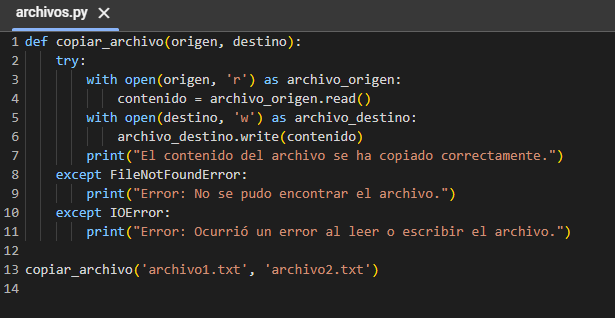
\includegraphics[width=4.0835in,height=2.1102in]{a0000-img002.png}}
\end{center}
\section[]{\rmfamily }
\section{cuenta bancaria}
\section[]{\rmfamily }
\section[]{\rmfamily }
\begin{center}
\lfbox[margin-right=0.1346in,margin-left=0.1252in,margin-top=0mm,margin-bottom=0mm,border-style=none,padding=0mm,vertical-align=top,raise=-0.2146in]{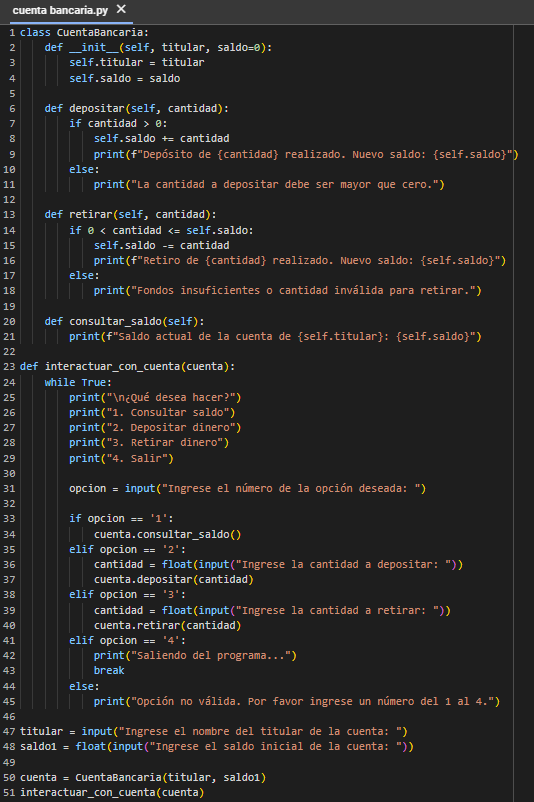
\includegraphics[width=3.552in,height=5.3346in]{a0000-img003.png}}
\end{center}

\bigskip
\bigskip


\bigskip


\bigskip


\bigskip
\bigskip


\bigskip


\bigskip


\bigskip
\section{Factorial}


\begin{center}
\lfbox[margin-right=0.1252in,margin-bottom=0.0043in,margin-left=0.1252in,margin-top=0mm,border-style=none,padding=0mm,vertical-align=top,raise=-0.2252in]{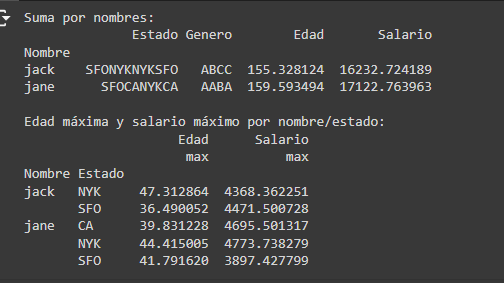
\includegraphics[width=3.9165in,height=1.2665in]{a0000-img004.png}}
\end{center}
\section[]{\rmfamily }
\section{Invertircadena}
\section[]{
\begin{center}
\lfbox[margin-right=0.1252in,margin-bottom=0.0055in,margin-left=0.1252in,margin-top=0mm,border-style=none,padding=0mm,vertical-align=top,raise=-0.2626in]{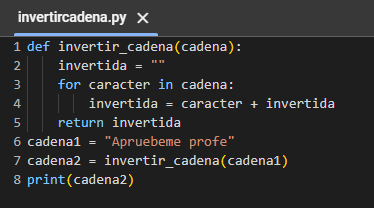
\includegraphics[width=3.25in,height=1.8071in]{a0000-img006.png}}
\end{center}
\section{Listatelefonica}
\section[]{\rmfamily }
\rmfamily }
\begin{center}
\lfbox[margin-right=0.1272in,margin-left=0.1252in,margin-top=0mm,margin-bottom=0mm,border-style=none,padding=0mm,vertical-align=top,raise=-2.6189in]{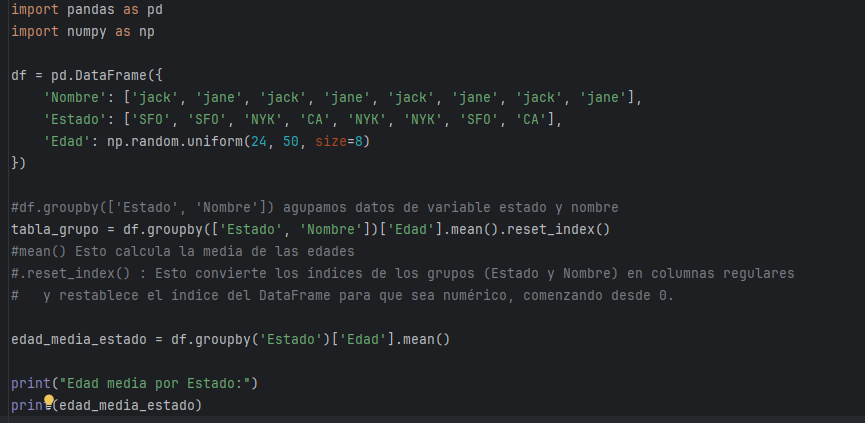
\includegraphics[width=3.7272in,height=4.5854in]{a0000-img005.png}}
\end{center}
\section{Parte 2: }
\section{Adivinar}
\begin{center}
\lfbox[margin-right=0.1252in,margin-bottom=0.0102in,margin-left=0.1252in,margin-top=0mm,border-style=none,padding=0mm,vertical-align=top,raise=-0.3654in]{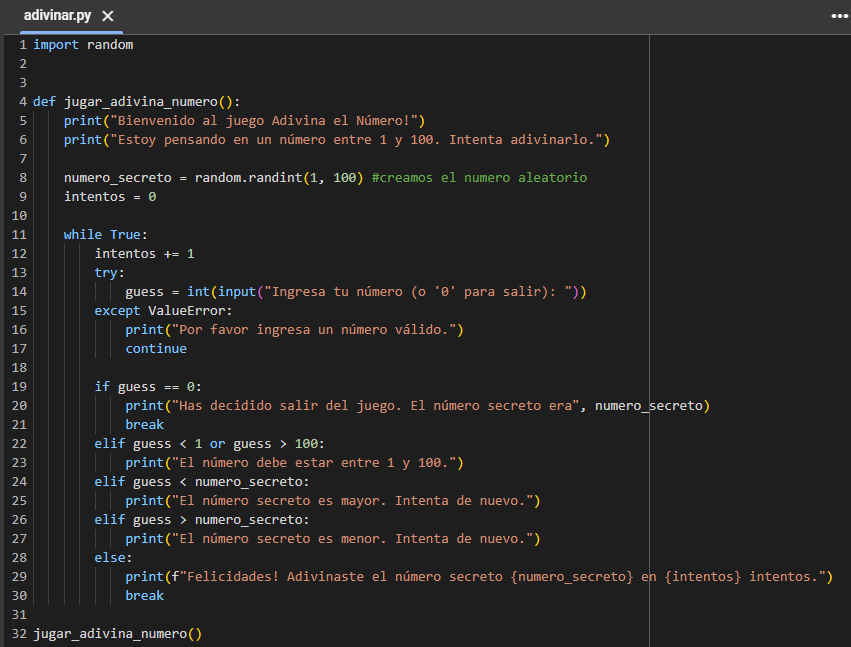
\includegraphics[width=4.4252in,height=3.3646in]{a0000-img007.png}}
\end{center}
\section[]{\rmfamily }
\section{Calculadora}
\begin{center}
\lfbox[margin-right=0.1252in,margin-left=0.1252in,margin-top=0mm,margin-bottom=0mm,border-style=none,padding=0mm,vertical-align=top,raise=-0.2618in]{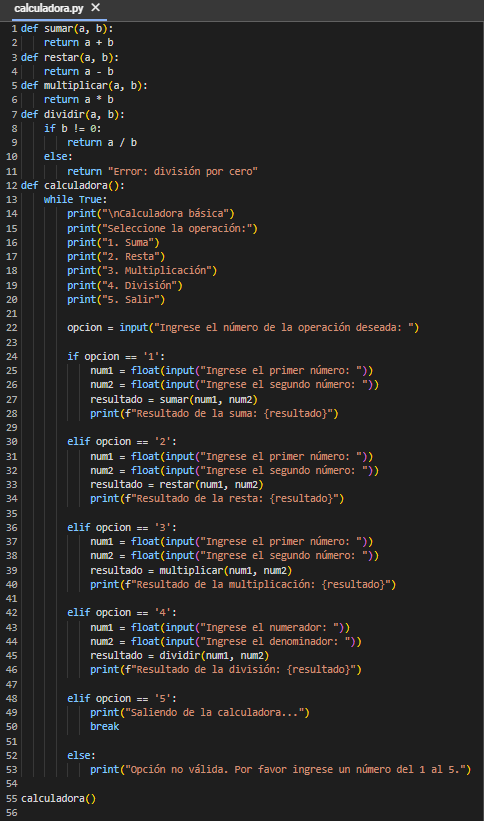
\includegraphics[width=2.8465in,height=4.8283in]{a0000-img008.png}}
\end{center}
\bigskip


\bigskip


\bigskip
\bigskip


\bigskip


\bigskip
\bigskip


\bigskip


\bigskip
\bigskip


\bigskip


\bigskip
\bigskip


\bigskip


\bigskip
\section{Cambiomoneda}
\section[]{\rmfamily }

\section[]{\rmfamily }
\begin{center}
\lfbox[margin-right=0.1256in,margin-bottom=0.0063in,margin-left=0.1252in,margin-top=0mm,border-style=none,padding=0mm,vertical-align=top,raise=-0.35in]{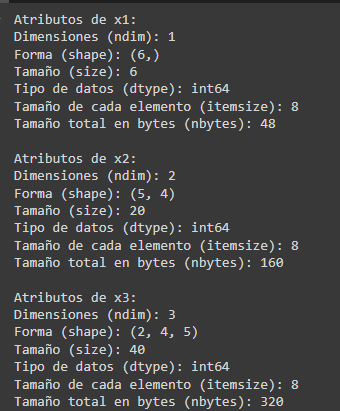
\includegraphics[width=7.7909in,height=6.7646in]{a0000-img009.png}}
\end{center}


\section{tareas4}
\section[]{\rmfamily }
\begin{center}
\lfbox[margin-right=0.1346in,margin-bottom=0.0098in,margin-left=0.1252in,margin-top=0mm,border-style=none,padding=0mm,vertical-align=top,raise=-0.2291in]{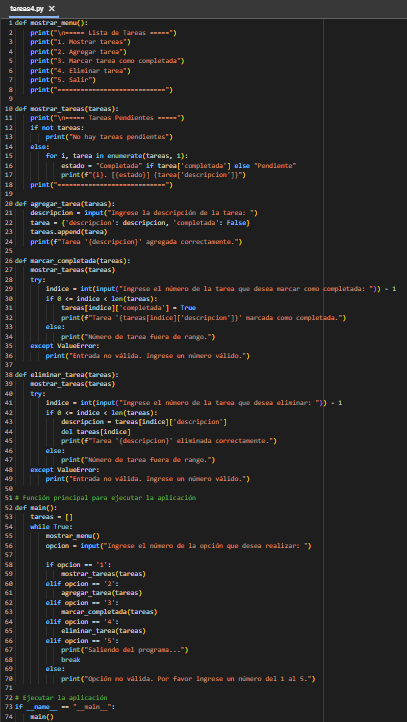
\includegraphics[width=4.8654in,height=8.6362in]{a0000-img010.png}}
\end{center}
\section[]{\rmfamily }
\section{Parte 3: }
\section{Punto1}
\section{Matplotlib(1)}
\begin{center}
\lfbox[margin-right=0.1311in,margin-bottom=0.0071in,margin-left=0.1252in,margin-top=0mm,border-style=none,padding=0mm,vertical-align=top,raise=-0.198in]{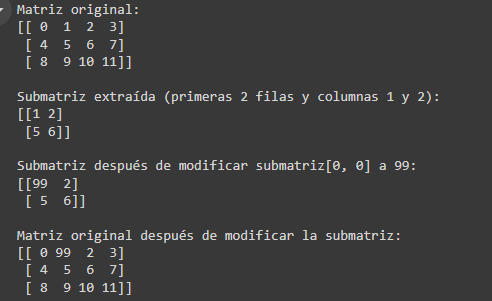
\includegraphics[width=2.2854in,height=1.0138in]{a0000-img011.png}}
\end{center}
\section[Numpy(2)]{\foreignlanguage{spanish}{Numpy(2)}}
\begin{center}
\lfbox[margin-right=0.1252in,margin-left=0.1252in,margin-top=0mm,margin-bottom=0mm,border-style=none,padding=0mm,vertical-align=top,raise=-1.2783in]{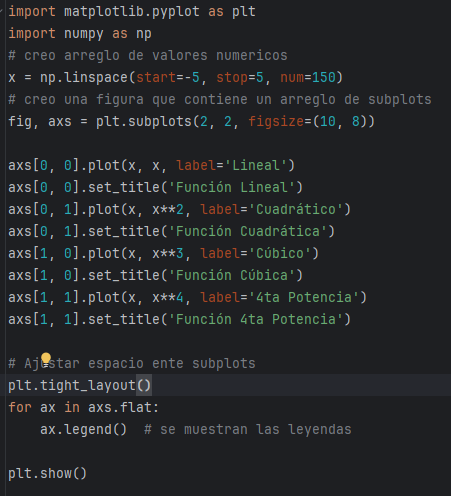
\includegraphics[width=3.9402in,height=3.3008in]{a0000-img012.png}}
\end{center}
\section[Panda(2)]{\foreignlanguage{spanish}{Panda(2)}}
\begin{center}
\lfbox[margin-right=0.1256in,margin-bottom=0.0016in,margin-left=0.1252in,margin-top=0mm,border-style=none,padding=0mm,vertical-align=top,raise=-3.6181in]{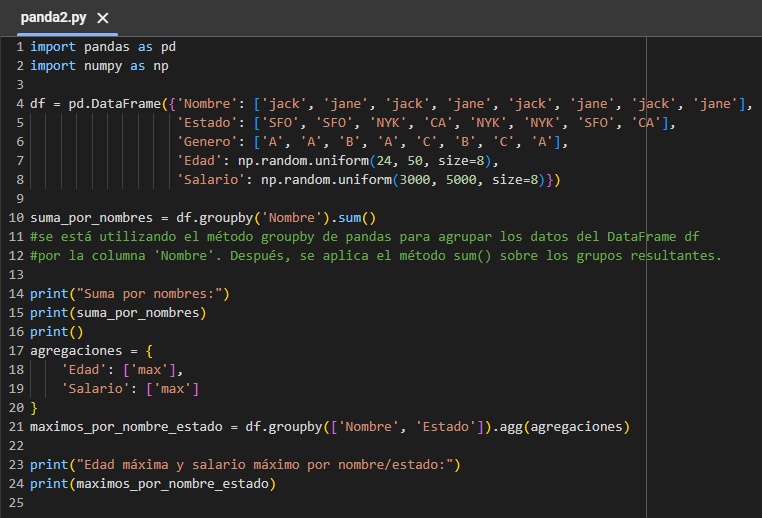
\includegraphics[width=5.2075in,height=3.5402in]{a0000-img013.png}}
\end{center}
\section[]{\selectlanguage{spanish}\rmfamily }
\bigskip


\bigskip


\bigskip

\bigskip
\bigskip


\bigskip


\bigskip


\section[Punto2]{\foreignlanguage{spanish}{Parte2}}
\section[\ Scikit{}-Learn(diabetes)]{\foreignlanguage{spanish}{\ Scikit-Learn(diabetes)}}

\begin{center}
\lfbox[margin-right=0.1283in,margin-bottom=0.0016in,margin-left=0.1252in,margin-top=0mm,border-style=none,padding=0mm,vertical-align=top,raise=-0.2508in]{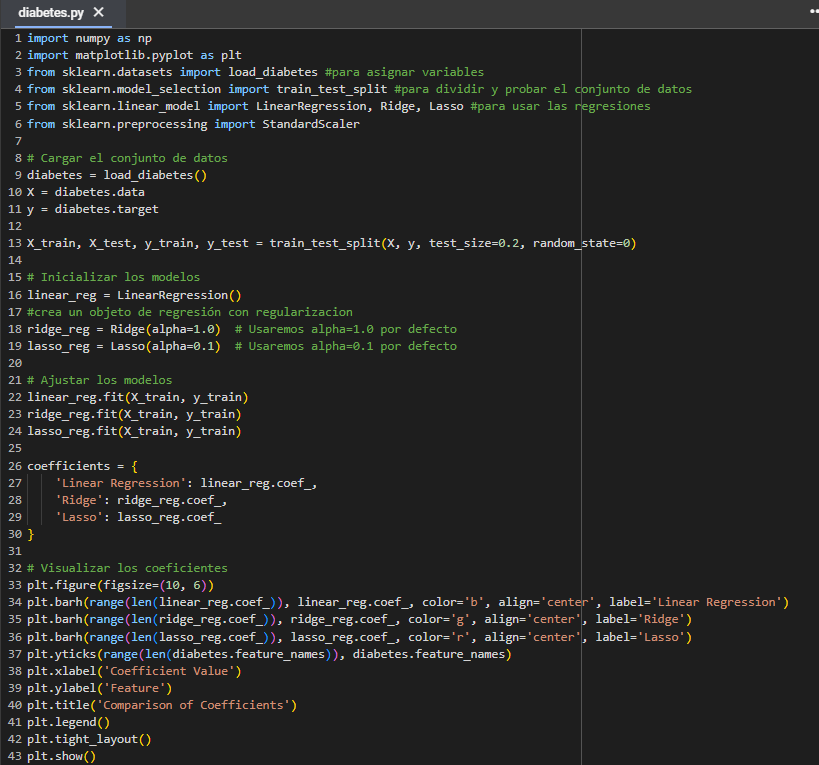
\includegraphics[width=5.8881in,height=5.4989in]{a0000-img014.png}}

\end{center}
\section[]{\selectlanguage{spanish}\rmfamily }

\section{Punto3}
\section{Clasificación(2)}
\section[]{\rmfamily }

\section[]{\rmfamily }
\begin{center}
\lfbox[margin-right=0.1252in,margin-left=0.1252in,margin-top=0mm,margin-bottom=0mm,border-style=none,padding=0mm,vertical-align=top,raise=-0.3744in]{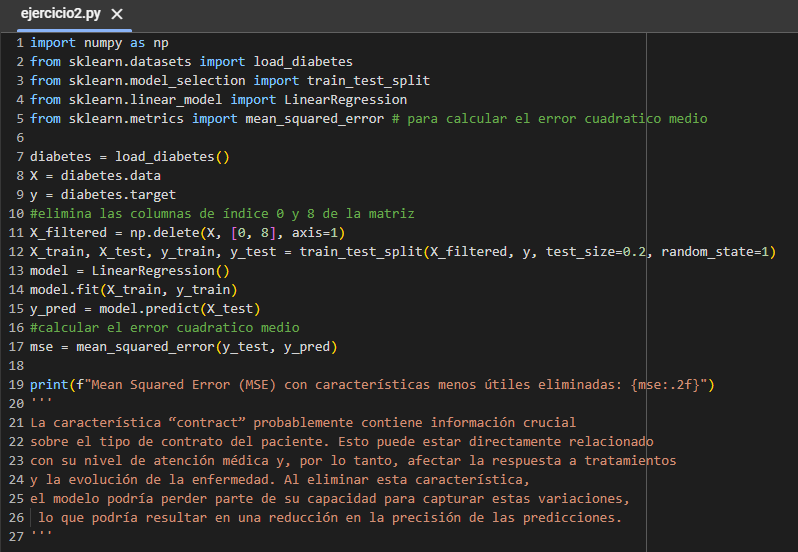
\includegraphics[width=8.0472in,height=5.5665in]{a0000-img015.png}}
\end{center}
\section[]{\rmfamily }
\section{Punto4}
\section{Metricas de clasificacion(4)}
\section[]{\rmfamily }

\bigskip



\begin{center}
\lfbox[margin-right=0.1335in,margin-left=0.1252in,margin-top=0mm,margin-bottom=0mm,border-style=none,padding=0mm,vertical-align=top,raise=-0.2807in]{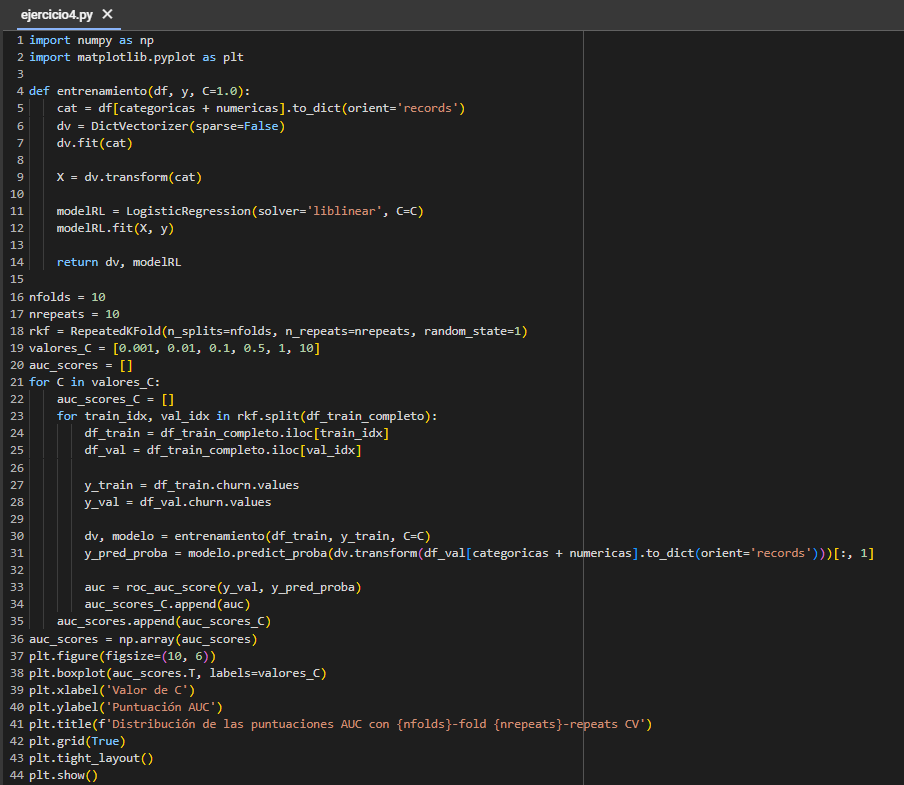
\includegraphics[width=7.9709in,height=6.9217in]{a0000-img016.png}}
\end{center}

\bigskip


\bigskip


\bigskip


\bigskip


\bigskip


\bigskip

\section{Punto5}
\section{Generación de textos(ejercicio dentro de la teoria)}
\section[]{\rmfamily }
\begin{center}
\lfbox[margin-right=0.1252in,margin-left=0.1252in,margin-top=0mm,margin-bottom=0mm,border-style=none,padding=0mm,vertical-align=top,raise=-0.4807in]{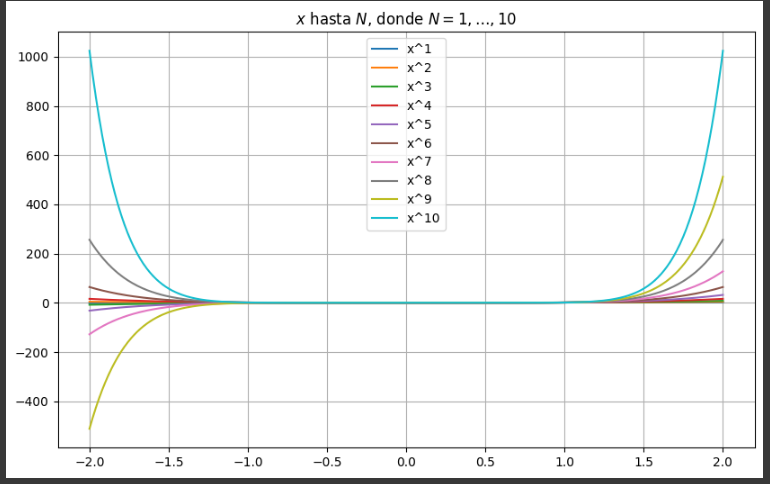
\includegraphics[width=8.0717in,height=6.8571in]{a0000-img017.png}}
\end{center}
\section{Punto6}

\section{Flask}
\begin{center}
\lfbox[margin-right=0.1252in,margin-left=0.1252in,margin-top=0mm,margin-bottom=0mm,border-style=none,padding=0mm,vertical-align=top,raise=-0.3453in]{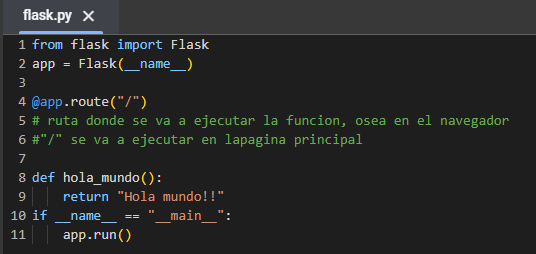
\includegraphics[width=4.8827in,height=2.3138in]{a0000-img018.png}}
\end{center}
\section{}
\section{Punto7}
\section{Proyecto}
\section{}
\begin{center}
\lfbox[margin-right=0.1252in,margin-left=0.1252in,margin-top=0mm,margin-bottom=0mm,border-style=none,padding=0mm,vertical-align=top,raise=-0.1965in]{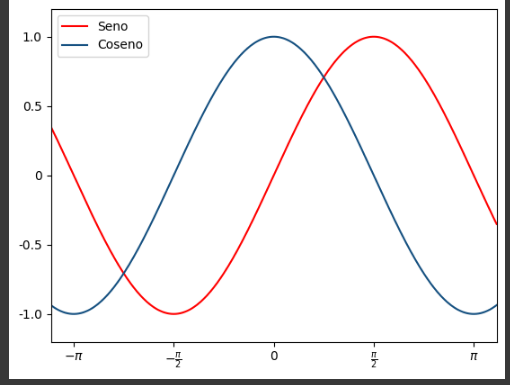
\includegraphics[width=5.4799in,height=5.4189in]{a0000-img019.png}}
\end{center}
\end{document}
